\documentclass[a4paper,12pt]{article}
\usepackage[english]{babel}
\usepackage[utf8]{inputenc}
\usepackage[T1]{fontenc}
\usepackage{enumitem}
\usepackage{amsmath,amssymb}
\usepackage{geometry}
\geometry{left=25mm,right=25mm,top=25mm,bottom=25mm}
\usepackage{parskip}

\usepackage{tikz}
\usetikzlibrary{circuits.ee.IEC, positioning}

\newif\ifshowsolutions
\showsolutionstrue  % comment to hide solutions

\begin{document}

\begin{center}
  {\LARGE\bfseries Introduction to Electrical Engineering \\[6pt] Practice Exam}\\[12pt]
  {\large Discussion: January 12, 2026}\\[6pt]
  \rule{\textwidth}{0.4pt}
\end{center}

\section{Conceptual Understanding: Multiple Choice}

Select exactly one answer per question.

\vspace{8pt}

\begin{enumerate}[label=\textbf{\arabic*.}, leftmargin=*, itemsep=8pt]

  \item The drift motion of electrons in a conductor is mainly caused by:
    \begin{itemize}[label=$\square$]
      \item[A)] temperature gradients
      \item[B)] applied magnetic fields
      \item[C)] an external electric field
      \item[D)] mechanical forces
    \end{itemize}

\ifshowsolutions
Solution: C
\fi

  \item For a metallic conductor, an increase in temperature usually leads to:
    \begin{itemize}[label=$\square$]
      \item[A)] decreasing resistance
      \item[B)] sudden insulating behavior
      \item[C)] unchanged resistance
      \item[D)] increasing resistance
    \end{itemize}

\ifshowsolutions
Solution: D
\fi

  \item Kirchhoff’s current law states:
    \begin{itemize}[label=$\square$]
      \item[A)] The sum of voltages in a loop is zero.
      \item[B)] The sum of currents at a node is zero.
      \item[C)] The sum of resistances at a node is constant.
      \item[D)] Power is stored at a node.
    \end{itemize}

\ifshowsolutions
Solution: B
\fi

  \item An ideal voltage source is characterized by:
    \begin{itemize}[label=$\square$]
      \item[A)] a fixed voltage independent of current
      \item[B)] a fixed current independent of the load
      \item[C)] infinite internal resistance
      \item[D)] no influence on connected circuits
    \end{itemize}

\ifshowsolutions
Solution: A
\fi

  \item The nodal-voltage method primarily works with:
    \begin{itemize}[label=$\square$]
      \item[A)] mesh currents
      \item[B)] node voltages
      \item[C)] equivalent sources
      \item[D)] frequency analysis
    \end{itemize}

\ifshowsolutions
Solution: B
\fi

  \item For maximum power transfer from a source to a purely resistive load:
    \begin{itemize}[label=$\square$]
      \item[A)] load resistance $>$ source internal resistance
      \item[B)] load resistance $<$ source internal resistance
      \item[C)] load resistance $=$ source internal resistance
      \item[D)] load resistance equals zero
    \end{itemize}

\ifshowsolutions
Solution: C
\fi

  \item An ammeter is typically connected:
    \begin{itemize}[label=$\square$]
      \item[A)] in parallel with the measured quantity
      \item[B)] in series with the measured quantity
      \item[C)] with zero internal resistance
      \item[D)] only in DC circuits
    \end{itemize}

\ifshowsolutions
Solution: B
\fi

  \item A capacitor primarily stores:
    \begin{itemize}[label=$\square$]
      \item[A)] magnetic energy
      \item[B)] mechanical energy
      \item[C)] thermal energy
      \item[D)] electric energy
    \end{itemize}

\ifshowsolutions
Solution: D
\fi

  \item Under constant DC voltage, a capacitor behaves (in steady state) like:
    \begin{itemize}[label=$\square$]
      \item[A)] a short circuit
      \item[B)] an open circuit
      \item[C)] a resistor with fixed value
      \item[D)] a voltage source
    \end{itemize}

\ifshowsolutions
Solution: B
\fi

  \item Magnetic fields are mainly generated by:
    \begin{itemize}[label=$\square$]
      \item[A)] stationary charges
      \item[B)] moving charges or electric current
      \item[C)] temperature changes
      \item[D)] light radiation
    \end{itemize}

\ifshowsolutions
Solution: B
\fi

  \item A conducting loop is located in a magnetic field that is constant in time. Electrical induction occurs when:
    \begin{itemize}[label=$\square$]
      \item[A)] the loop rotates
      \item[B)] the loop remains at rest
      \item[C)] the magnetic field is homogeneous
      \item[D)] the electrical resistance of the loop increases
    \end{itemize}

\ifshowsolutions
Solution: A
\fi

  \item Why can the current through an ideal inductor not change abruptly?
    \begin{itemize}[label=$\square$]
      \item[A)] Because the magnetic energy of the inductor would become infinite for a sudden change in current.
      \item[B)] Because an abrupt change in current would require an infinite induced voltage.
      \item[C)] Because magnetic fields cannot be established instantaneously.
      \item[D)] Because the inductance depends on the current.
    \end{itemize}

\ifshowsolutions
Solution: B
\fi

  \item An ideal transformer can:
    \begin{itemize}[label=$\square$]
      \item[A)] convert DC voltage to different DC voltage
      \item[B)] convert AC voltage to AC voltage with different amplitude
      \item[C)] permanently change the frequency of AC voltage
      \item[D)] generate energy
    \end{itemize}

\ifshowsolutions
Solution: B
\fi

  \item A transient process in an electrical network is characterized by:
    \begin{itemize}[label=$\square$]
      \item[A)] an algebraic equation without time dependence
      \item[B)] a first-order homogeneous differential equation with an exponential solution
      \item[C)] the absence of energy storage elements
      \item[D)] a time-invariant (constant) state
    \end{itemize}

\ifshowsolutions
Solution: B
\fi

  \item In which situation is the phasor representation of a current \emph{not} applicable?
    \begin{itemize}[label=$\square$]
      \item[A)] for a sinusoidal current with constant frequency
      \item[B)] in the steady-state of a linear network
      \item[C)] during an exponentially decaying transient
      \item[D)] for an AC voltage with fixed angular frequency
    \end{itemize}

\ifshowsolutions
Solution: C
\fi

  \item The reactance of a capacitor decreases with increasing frequency:
    \begin{itemize}[label=$\square$]
      \item[A)] increases
      \item[B)] decreases
      \item[C)] remains constant
      \item[D)] is unpredictable
    \end{itemize}

\ifshowsolutions
Solution: B
\fi

  \item Reactive power occurs in an AC circuit when:
    \begin{itemize}[label=$\square$]
      \item[A)] voltage and current are phase-shifted
      \item[B)] voltage and current are exactly in phase
      \item[C)] no energy is transferred
      \item[D)] only DC current flows
    \end{itemize}

\ifshowsolutions
Solution: A
\fi

  \item A high-pass filter ideally allows:
    \begin{itemize}[label=$\square$]
      \item[A)] low frequencies
      \item[B)] high voltages
      \item[C)] DC only
      \item[D)] high frequencies
    \end{itemize}

\ifshowsolutions
Solution: D
\fi

  \item Resonance in a series resonant circuit means:
    \begin{itemize}[label=$\square$]
      \item[A)] minimum impedance
      \item[B)] maximum damping
      \item[C)] no load influence
      \item[D)] instantaneous decay
    \end{itemize}

\ifshowsolutions
Solution: A
\fi

  \item A practical advantage of a symmetrical three-phase system is:
    \begin{itemize}[label=$\square$]
      \item[A)] lower frequency
      \item[B)] only two conductors are required
      \item[C)] generation of a rotating magnetic field in electric machines
      \item[D)] no balancing current possible
    \end{itemize}

\ifshowsolutions
Solution: C
\fi

\end{enumerate}

\newpage

\section{DC Networks}

\subsection{Equivalent Resistance}

Given the resistor network with $R_1 = 10\,\Omega$, $R_2 = 20\,\Omega$, $R_3 = 30\,\Omega$, $R_4 = 5\,\Omega$, $R_5 = 15\,\Omega$:

\begin{center}
\begin{tikzpicture}[circuit ee IEC, scale=1]
% Left terminal A
\draw (0,0) node[left]{A} -- (1,0);
% R1 in series
\draw (1,0) to[resistor={info=$R_1$}] (3,0);
% Split node
\draw (3,0) -- (4,0);
\draw (4,0) -- (4,2);
% Upper branch: R2 and R3 in series
\draw (4,2) to[resistor={info=$R_2$}] (6,2)
           to[resistor={info=$R_3$}] (8,2)
           -- (8,0);
% Lower branch: R4
\draw (4,0) to[resistor={info=$R_4$}] (8,0);
% Continue in series with R5
\draw (8,0) -- (9,0)
      to[resistor={info=$R_5$}] (11,0)
      -- (12,0);
% Right terminal B
\draw (12,0) node[right]{B};
\end{tikzpicture}
\end{center}

Calculate the equivalent resistance of the network.

\ifshowsolutions
Solution:
\[
R_{23} = R_2 + R_3 = 20 + 30 = 50\,\Omega
\]
\[
\frac{1}{R_{234}} = \frac{1}{R_{23}} + \frac{1}{R_4} = \frac{1}{50} + \frac{1}{5} = \frac{11}{50}
\]
\[
R = R_1 + R_{234} + R_5 = 10 + \frac{50}{11} + 15 = 29.55\,\Omega
\]
\fi

\subsection{Network Analysis}

Given the circuit with $R_1 = 6\,\Omega$, $R_2 = 12\,\Omega$, $R_3 = 4\,\Omega$ and a voltage source of $24\,\mathrm{V}$:

\begin{center}
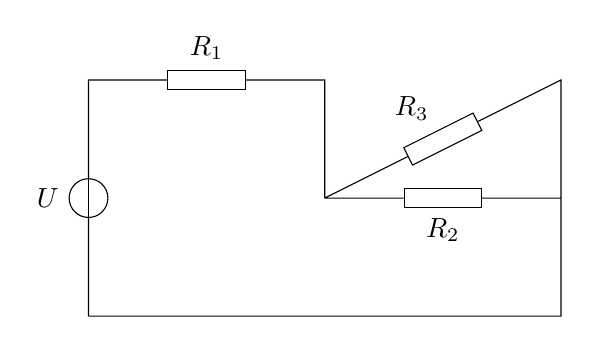
\begin{tikzpicture}[circuit ee IEC]
  \draw
  (0,0) to[voltage source={info={$U$}}] (0,3)
        to[resistor={info={$R_1$}}] (3,3)
        -- (3,1.5)
  (3,1.5) to[resistor={info'={$R_2$}}] (6,1.5)
        -- (6,0)
  (3,1.5) to[resistor={info={$R_3$}}] (6,3)
        -- (6,0) -- (0,0);
\end{tikzpicture}
\end{center}

Determine:

\begin{enumerate}
  \item the total source current,
  \item the branch currents through $R_2$ and $R_3$,
  \item the power dissipated in $R_3$.
\end{enumerate}

\ifshowsolutions
Solution:
\[
R_{23} = \frac{12 \cdot 4}{16} = 3\,\Omega
\]
\[
R = 6 + 3 = 9\,\Omega
\]
\[
I = \frac{24}{9} = 2.67\,\text{A}
\]
\[
U_{23} = I \cdot 3 = 8\,\text{V}
\]
\[
I_2 = \frac{8}{12} = 0.67\,\text{A}, \quad I_3 = \frac{8}{4} = 2\,\text{A}
\]
\[
P_3 = I_3^2 R_3 = 16\,\text{W}
\]
\fi

\subsection{Nodal Analysis}

Given the DC network with $U = 20\,\mathrm{V}$, $R_1 = 5\,\Omega$, $R_2 = 10\,\Omega$, $C = 100\,\mu\mathrm{F}$:

\begin{center}
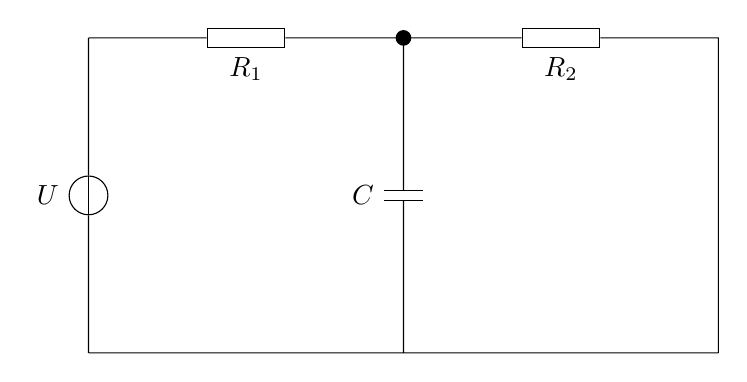
\begin{tikzpicture}[circuit ee IEC, scale=1]
  \draw
  % Spannungsquelle
  (0,0) to[voltage source={info={$U$}}] (0,4)

  % R1
  (0,4) to[resistor={info'={$R_1$}}] (4,4)

  % Knoten
  (4,4) node[circle,fill,inner sep=2pt] {}

  % R2
  (4,4) to[resistor={info'={$R_2$}}] (8,4)
        -- (8,0)

  % Kondensator
  (4,4) to[capacitor={info'={$C$}}] (4,0)

  % Masse
  (0,0) -- (8,0);
\end{tikzpicture}
\end{center}

The lower conductor is chosen as reference potential (ground). The steady-state condition ($t \rightarrow \infty$) is assumed.

Determine:

\begin{enumerate}
  \item the node voltage at the marked node,
  \item the voltage across the capacitor,
  \item the current through the capacitor,
  \item the energy stored in the capacitor.
\end{enumerate}

\ifshowsolutions
Solution:
\[
\frac{V_1 - 20}{R_1} + \frac{V_1 - 0}{R_2} = 0
\]
\[
2(V_1 - 20) + V_1 = 0
\]
\[
V_1 = \frac{40}{3} \approx 13.33\,\text{V}
\]
\[
U_C = V_1 - 0 = 13.33\,\text{V}
\]
\[
i_C = C \frac{du_C}{dt} = 0
\]
\[
W = \frac{1}{2} C U_C^2 \approx 8.9\,\text{mJ}
\]
\fi

\newpage

\section{AC Networks}

\subsection{Equivalent Impedance}

Given the AC network with  $R_1 = 10\,\Omega$, $R_2 = 20\,\Omega$, $L = 50\,\mathrm{mH}$, $C = 100\,\mu\mathrm{F}$, $\omega = 1000\,\mathrm{rad/s}$:

\begin{center}
\begin{tikzpicture}[circuit ee IEC, scale=1]
  \draw
  % Eingang
  (0,0) node[left]{A}
  to[resistor={info'={$R_1$}}] (3,0)

  % Parallelschaltung
  (3,0) -- (3,2)
  to[inductor={info'={$L$}}] (6,2)
  -- (6,0)

  (3,0) -- (3,-2)
  to[capacitor={info'={$C$}}] (6,-2)
  -- (6,0)

  % R2
  to[resistor={info'={$R_2$}}] (9,0)
  node[right]{B};
\end{tikzpicture}
\end{center}

Determine:

\begin{enumerate}
  \item the complex impedances of the individual components,
  \item the complex equivalent impedance between terminals A and B,
  \item the magnitude and phase of the equivalent impedance.
\end{enumerate}

\ifshowsolutions
Solution:
\[
\underline{Z}_R = R
\]
\[
\underline{Z}_L = j \omega L = j \cdot 1000 \cdot 0.05 = j50\,\Omega
\]
\[
\underline{Z}_C = \frac{1}{j \omega C} = \frac{1}{j \cdot 1000 \cdot 100 \cdot 10^{-6}} = -j10\,\Omega
\]
\[
\underline{Z}_{LC} = \left( \frac{1}{Z_L} + \frac{1}{Z_C} \right)^{-1} = \frac{1}{j0.08} = -j12.5\,\Omega
\]
\[
\underline{Z} = R_1 + Z_{LC} + R_2 = (30 - j12.5)\,\Omega
\]
\[
|\underline{Z}| = \sqrt{30^2 + 12.5^2} \approx 32.5\,\Omega
\]
\[
\varphi = \arctan\left(\frac{-12.5}{30}\right) \approx -22.6^\circ
\]
\fi

\subsection{Complex Network Analysis}

Given the following network with a sinusoidal voltage source $U = 230\,\mathrm{V}$, $f = 50\,\mathrm{Hz}$ and the components $R = 20\,\Omega$, $L = 100\,\mathrm{mH}$:

\begin{center}
\begin{tikzpicture}[circuit ee IEC]
  \draw
  (0,0) to[voltage source={info={$U$}}] (0,3)
        to[resistor={info={$R$}}] (3,3)
        to[inductor={info={$L$}}] (6,3)
        -- (6,0) -- (0,0);
\end{tikzpicture}
\end{center}

Determine:

\begin{enumerate}
  \item the complex impedance $Z$,
  \item the RMS current $I$,
  \item the phase shift between current and voltage,
  \item the power factor $\cos\varphi$,
  \item the active power $P$,
  \item the reactive power $Q$.
\end{enumerate}

\ifshowsolutions
Solution:
\[
\omega = 2\pi f = 314\,\text{rad/s}
\]
\[
X_L = \omega L = 31.4\,\Omega
\]
\[
\underline{Z} = 20 + j31.4 \Rightarrow |Z| = 37.3\,\Omega
\]
\[
I = \frac{230}{37.3} = 6.17\,\text{A}
\]
\[
\varphi = \arctan\left(\frac{31.4}{20}\right) = 57.5^\circ
\]
\[
\cos\varphi = 0.54
\]
\[
P = U I \cos\varphi = 766\,\text{W}
\]
\[
Q = U I \sin\varphi = 1180\,\text{var}
\]
\fi

\newpage

\section*{Formula Sheet}

\subsection*{Capacitor}

\[
i_C(t) = C \frac{du_C(t)}{dt}
\]

\[
W = \frac{1}{2} C U^2
\]

\subsection*{AC}

\[
\omega = 2 \pi f
\]

\[
\underline{Z}_L = j \omega L
\]

\[
\underline{Z}_C = \frac{1}{j \omega C}
\]

\[
\underline{Z} = R + jX
\]

\[
P = U I \cos \varphi
\]

\[
Q = U I \sin \varphi
\]

\end{document}